\documentclass[9pt]{article}
\usepackage{amsmath, amsthm}
\usepackage{graphicx}
\usepackage{url} 

\title{MAE 250F Final Project - Equilibrium Air Flow Across a Hypersonic Shock Wave}
\author{Hrafnkell Palsson}
\date{March 15, 2010}

\begin{document}
\maketitle

% An example comment.
\section*{Introduction of technical problem}
The objective of this paper is to recreate fig. 14.4a and 14.4b page 609, and fig. 14.5a and 14.5b page 610 of Anderson's Hypersonic and High-Temperature Gas Dynamics [4]. Anderson, in turn, obtained these figures from a 1963 NASA Technical Report by P. W. Huber [1]. Figure 14.4 shows air temperature behind a normal shock as a function of upstream velocity. The air is modeled as real gas and the flow is assumed to be equilibrium flow. Under these assumptions the increase in temperature across the shock is not simply a function of the upstream Mach number, as is the case for perfect gas. Apart from the upstream velocity, the downstream properties also depend on upstream pressure and temperature (or in general, any two independent upstream thermodynamic variables). Every curve on figure 14.4 is drawn for a certain atmospheric height, considered to be at a fixed pressure and temperature. Figure 14.5 shows the density increase of air across a normal shock, under the same assumptions and at the same heights.

The reason the properties behind the normal shock are also a function of pressure and temperature is because the air is modeled as a chemically reacting real gas. The chemical composition of the air and the excitement of different energy modes, which affect the thermodynamic state of the air, depend on the pressure and the temperature of the mixture.

\section*{Governing equations}
The governing equations are the continuity, momentum and energy equations, and two equations describing the equilibrium thermodynamic properties of air ("equations of state").

\noindent Continuity:
\begin{equation}
\label{cont}
\rho_{1}*u_{1} = \rho_{2}*u_{2}
\end{equation}
Momentum:
\begin{equation}
\label{mom}
p_{1}+\rho_{1}*u_{1}^{2}=p_{2}+\rho_{2}*u_{2}^{2}
\end{equation}
Energy:
\begin{equation}
\label{energy}
h_{1}+\frac{u_{1}^{2}}{2}=p_{2}+\frac{u_{2}^{2}}{2}
\end{equation}

The equilibrium thermodynamic equations Huber [1] uses to create the figures are curve fits designed especially for equilibrium air by Tannehill and Mugge [2]. We will use a newer, improved version of those curve fits by Srinivasan, Tannehill and Weilmuenster [3]. They have created multiple curve fist and one can choose between a couple of them to recreate the figures. This paper uses $p=p(e,\rho)$ and $T=T(p,\rho)$.

\noindent The $p=p(e,\rho)$ curve fit is:
\begin{equation}
\label{p_correlation}
p=\rho*e*(\tilde{\gamma}-1) 
\end{equation}
where
\[
\begin{split}
\tilde{\gamma} =a_{1}+a_{2}*Y+a_{3}*Z+a_{4}*Y*Z+a_{5}*Y^{2}+\\
a_{6}*Z^{2}+a_{7}*Y^{2}*Z+a_{8}*Y*Z^{2}+a_{9}*Y^{3}+a_{10}*Z^{3}+\\
(a_{11}+a_{12}*Y+a_{13}*Z+a_{14}*Y*Z+a_{15}*Y^{2}\\
+a_{16}*Z^{2}+a_{17}*Y^{2}*Z+a_{18}*Y*Z^{2}+a_{19}*Y^{3}+a_{20}*Z^{3})\\
/(1\pm\exp(a_{21}+a_{22}*Y+a_{23}*Z+a_{24}*Y*Z)
\end{split}
\]
where $Y=\log(\frac{\rho}{\rho_{0}})$ and $Z=\log(\frac{e}{R*T_{0}})$.

\noindent The $T=p(p,\rho)$ curve fit is:
\begin{equation}
\label{T_correlation}
T=T_{0}*10^{\tilde{\gamma}}
\end{equation}
where
\[
\begin{split}
 \tilde{\gamma} =d_{1}+d_{2}*Y+d_{3}*Z+d_{4}*Y*Z+d_{5}*Y^{2}+\\
d_{6}*Z^{2}+d_{7}*Y^{2}*Z+d_{8}*Y*Z^{2}+d_{9}*Y^{3}+d_{10}*Z^{3}+\\
(d_{11}+d_{12}*Y+d_{13}*Z+d_{14}*Y*Z+d_{15}*Y^{2}\\
+d_{16}*Z^{2}+d_{17}*Y^{2}*Z+d_{18}*Y*Z^{2}+d_{19}*Y^{3}+d_{20}*Z^{3})\\
/(1\pm\exp(d_{21}+d_{22}*Y+d_{23}*Z+d_{24}*Y*Z)
\end{split}
\]
where $Y=\log(\frac{\rho}{\rho_{0}})$, $X=\log(\frac{p}{p_{0}})$ and $Z=X-Y$.

\section*{Description of calculation method}
\noindent We need to rewrite the continuity, momentum and energy equations to a suitable form to use in the calculation procedure.
\begin{equation}
\label{cont_mod}
u_{2}=\frac{\rho_{1}*u_{1}}{u_{2}}
\end{equation}
Inserting \eqref{cont_mod} into the \eqref{mom} and rearranging we get:
\begin{equation}
p_{2}=p_{1}+\rho_{1}*u_{1}^{2}(1-\frac{\rho_{1}}{\rho_{2}})
\end{equation}
Inserting \eqref{cont_mod} into \eqref{energy} and rearranging we get:
\begin{equation}
h_{2}=h_{1}+\frac{u_{1}^{2}}{2}(1-(\frac{\rho_{1}}{\rho_{2}})^{2})
\end{equation}
\noindent The calculation procedure for reproducing the figures then becomes:
\begin{enumerate}
\item Assume a value for $\rho_2$. $\rho_1$ is a known upstream value so this fixes the value of $\rho_{1}/\rho_{2}$.
\item Calculate $p_2$ from (7).
\item Calculate $h_2$ from (8).
\item With values of $p_2$ and $h_2$ just obtained, solve numerically for $\rho_2$ using (4). Note that $e=h-p/\rho$. This is an implicit equation for $\rho$ as function of $h$ and $p$.
\item Form a new value of $\rho_{1}/\rho_{2}$ using the value of $\rho_2$ just obtained.
\item Use this new value of $\rho_{1}/\rho_{2}$ to obtain new values of $p_2$ and $h_2$ just as in steps 2 and 3. Then repeat steps 2 to 6 until convergence is obtained, that is, until there is only a negligible change in $\rho_{1}/\rho_{2}$ from one iteration to the next.
\item At this stage, we now have the correct values of $p_2$, $h_2$ and $\rho_2$. Obtain the correct value of $T_2$ using (5).
\item Repeat the steps above for upstream pressure, temperatures and velocities required to reproduce the figures.
\item Note that the perfect gas law is assumed to be valid upstream.
\end{enumerate}

\section*{Input data and parameters}
The reference conditions $p_0$ and $T_0$ are obtained from [3]. $\rho_0$ is then calculated from the perfect gas law. The gas constant, $R$, and the specific heats, $c_p$ and $c_v$, were also needed for calculation of upstream properties. The pressures and temperatures for the altitudes on the figures are obtained from table IV in [1]. The values of the constants are:
\begin{align*}
p_{0}=101325Pa [1] \\
T_{0}=273.15K [1] \\
R = 287.058\tfrac{J}{kg*K} [5]\\
\rho_{0}=\tfrac{p_{0}}{R*T_{0}}=1.2922\tfrac{kg}{m^{3}} \\
c_p=1003.5\tfrac{J}{kg*K} [6] \\
\gamma=1.403\tfrac{J}{kg*K} [7] \\
c_{v} = c_{p}/\gamma=715.25\tfrac{J}{kg*K}
\end{align*}

\section*{Computation results}
The results of the computation are the recreated figures.
\begin{figure}[!htbp]
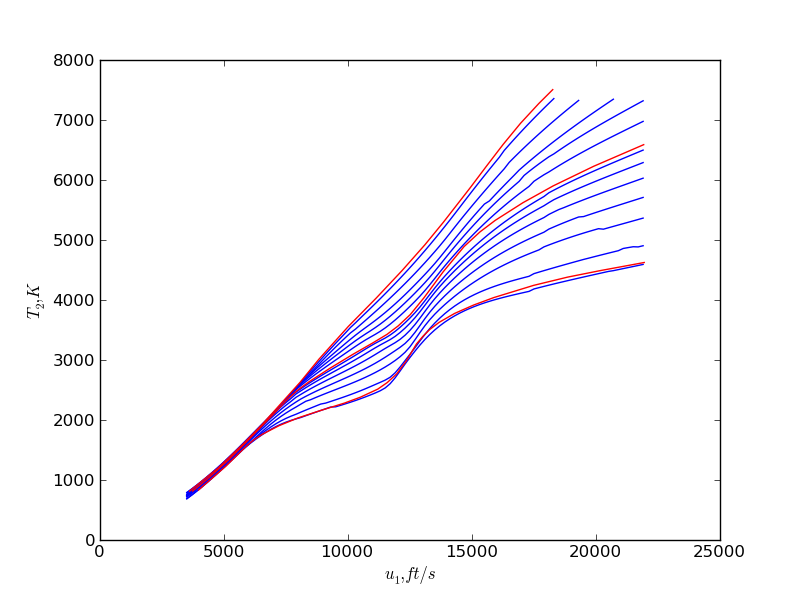
\includegraphics[width=0.80\textwidth]{144a}
\caption{Figure 14.4a. Variation of normal shock temperature with velocity and altitude; velocity range below orbital velocity.}
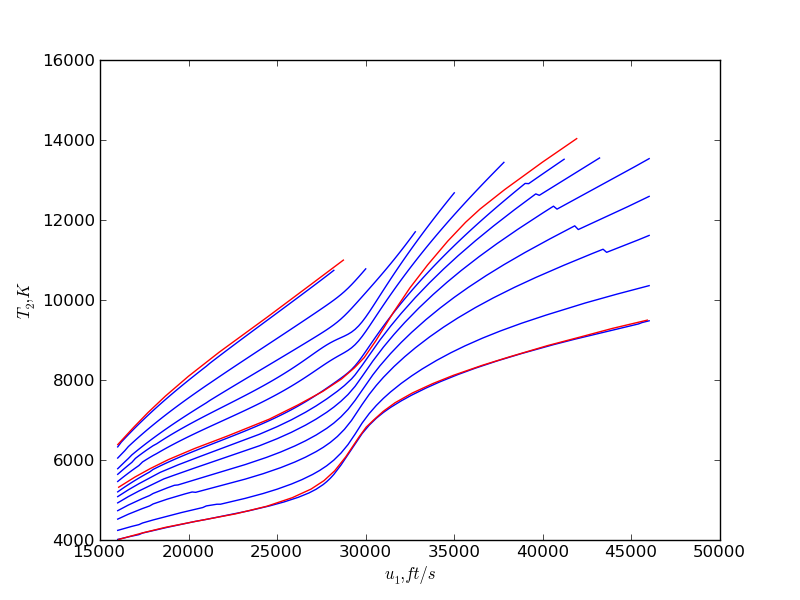
\includegraphics[width=0.80\textwidth]{144b}
\caption{Figure 14.4b. Variation of normal shock temperature with velocity and altitude; velocity range near and above orbital velocity.}
\end{figure}
\begin{figure}[!htbp]
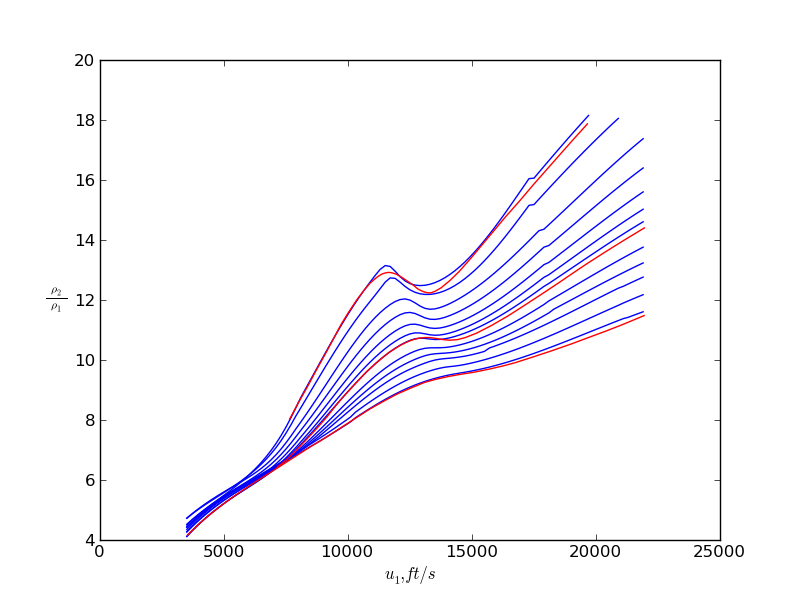
\includegraphics[width=0.80\textwidth]{145a}
\caption{Figure 14.5a. Variation of normal shock density with velocity and altitude; velocity range below orbital velocity.}
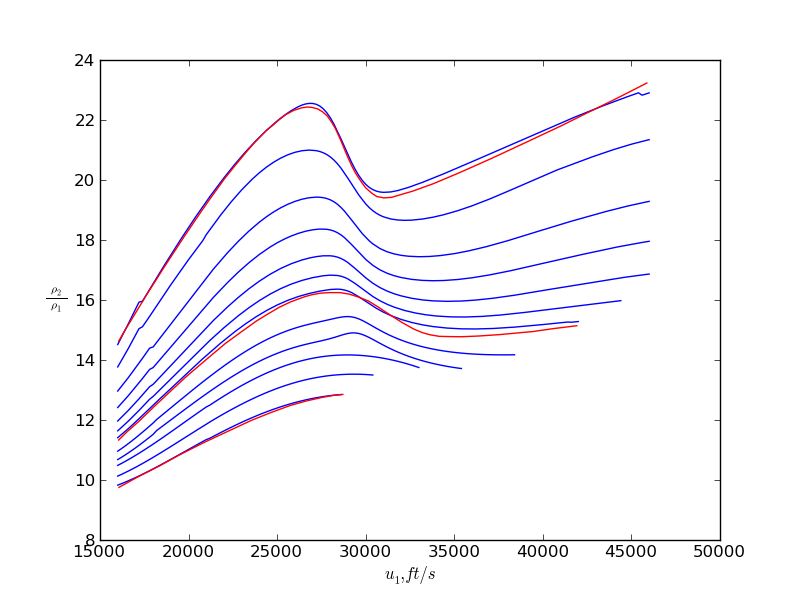
\includegraphics[width=0.80\textwidth]{145b}
\caption{Figure 14.5b. Variation of normal shock density with velocity and altitude; velocity range below orbital velocity.}
\end{figure}

\newpage
\section*{Discussion of results}
The reproduction of the figures from Anderson's book are reasonably accurate. The three red curves are curves from Anderson's book, obtained by digitization, using the software Engauge Digitizer [8] (three curves were chosen in order not to crowd the plotted figures). They are the 35.900 ft, 154.800 ft and the 322.900 ft curves. As mentioned previously, this paper does not use the same curve fits as Huber [1], so the slight shifting in the curves is to be expected. The kinks at many places in the plotted curves might be due to errors in the tables of constants, A.1-A.3 and A.10-A.12, in [3].

\section*{Conclusions}
The figures have been recreated, but not in a completely satisfactory manner. The source of the kinks has not been determined.

\section*{References}
\begin{enumerate}
\item P. W. Huber, "Hypersonic shock-heated flow parameters for velocities to 46,000 feet per second and altitudes to 323,000 feet," December 1963, NASA Technical Report.
\item J. C. Tannehill and P. H. Mugge, "Improved Curve Fits for the Thermodynamic Properties of Equilibrium Air Suitable for Numerical Computation Using Time-Dependent or Shock-Capturing Methods," NASA CR-2470, Oct. 1974.
\item S. Srinivasan, J. C Tannehill, and K. J Weilmuenster, "Simplified Curve Fits for the Thermodynamic Properties of Equilibrium Air," NASA RP-1181, 1987.
\item J. D. Anderson Jr., \textit{Hypersonic And High-Temperature Gas Dynamics}, 2nd ed., AIAA, Reston, Virginia, 2006.
\item "Gas Constant," \url{http://en.wikipedia.org/wiki/Gas_constant}
\item "Air Properties," \url{http://www.engineeringtoolbox.com/air-properties-d_156.html}
\item "Engauge Digitizer," \url{http://digitizer.sourceforge.net}
\end{enumerate}

% \bibliographystyle{plain}
% \bibliography{250f_final_project}

\end{document}
